\documentclass[10pt,twocolumn]{article} 

\usepackage{oxycomps} % use the main oxycomps style file

\bibliography{references}

\pdfinfo{
    /Title (Machine Learning And Crypto Currency)
    /Author (Haotian wang)
}

\title{Machine Learning And Crypto Currency}

\author{Haotian wang}
\affiliation{Occidental College}
\email{hwang2@oxy.edu}

\begin{document}

\maketitle

\begin{abstract}
   \end{abstract}

\section{Introduction}

\section{Problem Context}
	In researching and investing in both the stock market and the cryptocurrency market, several differences and issues were observed. Even though the stock market was known as unpredictable by the majority, economists and investors have examined a series of growth and decrease using past trend experiences. There is a Candlestick chart for the investors to take reference when people invest in the stock market. A candlestick chart is a technical tool that packs multiple times frames into a single price bar. As years passed, the professionalism has summarized a systematic pattern for different trends and analyzed their possibilities of growing and descending based on the standard candlestick chart.

	Meanwhile, in order to regular the stock market and provide a stabilized trading environment, the stock market only opens six and half hours on average Monday through Friday under the authorities' regulation. In addition, the authorities also analyzed a systematic candlestick chart pattern to monitor the abnormal situations on the stock market; Meaning that certain patterns can be used to see the possible trends. On the other hand, as cryptocurrencies are based on blockchain technology and consist of the central idea of decentralization, it becomes hard for the authorities to monitor and regulate the market. Without the regulations and authorities, monitoring results in unpredicted chaos in the market. In contrast to the stock market, the cryptocurrency market is unpredictable due to no regulation, 24/7 market time, and decentralization. 

	Each stock is being rated and investigated to unsure its credibility by the Securities and Exchange Commission and authorized stock exchange to ensure the safety of the market along with the investors and minimize the chance of scam by corporates using false background information. In contrast, the crypto market is unsupervised, and it leads to a trading environment with an easier scam using false background information. For instance, a team without accurate background information could write a smart contract on any blockchain using made-up information and project to allow investors to lose money. These scam cryptos can decrease the trust between investors and cause and scurviness trading environment. Last but not least, the more complicated cryptocurrency market could have a general systematic pattern not yet been discovered, and the unsupervised state can result in an overflow of scam cryptos. These problems could be solved by machine learning potentially. 

\section{Technical Background}
	Machine learning now is fundamentally different from machine learning in the past, thanks to advancements in computing technology. Researchers interested in artificial intelligence wanted to discover if computers could learn from data and were inspired by pattern recognition and the hypothesis that computers can learn without executing specific tasks. The iterative feature of machine learning is significant because models are exposed to new data and can adjust without human intervention. Machine learning models can learn from their prior computations and use this knowledge to make judgments and create trustworthy and predictable outcomes. Machine learning is chosen to solve the two issues listed above as these models are significantly sensitive to patterns in data. Both issues have one thing in common: there could be potential patterns helping investors make the right decision and avoid scams. They are four essential parts of using machine learning to solve these problems; Getting data from an open-source data center; feeding old data into the machine learning algorithm; allowing the model to be trained using these data; summarize different patterns.

	With that being said, Pattern recognition is proposed as a solution. Pattern recognition is achieved by utilizing the concept of learning. Learning allows the pattern recognition system to be trained and become flexible, allowing it to offer more accurate findings due to its experience. Approximately one-third of the data set is used for training the system, with the remaining third being used for testing. figure1 shows how data is used for training and testing. The training set is a collection of images or data used to train or develop a machine learning model. Training rules are used to establish the criteria for making output judgments, then implemented. Training techniques are employed to match a given set of input data with a corresponding set of output decisions. The algorithms and rules are then put into action in order to make training more efficient. In order to generate results, the system makes use of the information gathered from the data. The testing set is used to determine whether or not the system is accurate. After the system has been trained, the testing data is used to determine whether or not the accurate output has been achieved. It is estimated that this data makes up around 20 percent of all the data in the pattern recognition system in question.

\begin{figure}
    \centering
    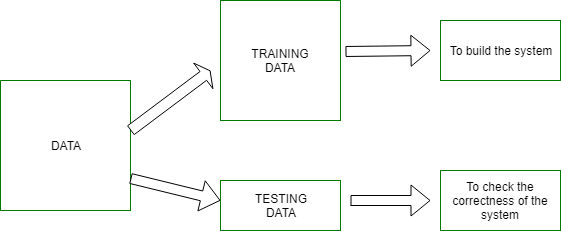
\includegraphics[width=.95\linewidth]{training-and-testing.png}
    \caption{
        pattern recognition process
    }
    \label{fig:first-page}
\end{figure}
	This project chooses to use Neural network-based algorithms as the main algorithm to build the model. these algorithms form a model that consists of parallel structures. Neural network have a well known learning abilities. Neural networks are algorithms inspired by the neurons that exist in human brains. A pattern recognition algorithm is meant to recognize patterns in large amounts of complex data. It frequently performs best when recognizing sounds, photos, or video patterns. Neurons are interconnected. A neural network is nothing more than a collection of neurons (also called nodes). These nodes are all linked together in some way. Then each neuron is associated with a number, and each connection is associated with a weight. These neurons are divided into three layers: the input, hidden, and output layers. There are numerous layers, and there is no universally accepted optimal number of layers. figure 2 demonstrates the structure of theses three layers. The input layer represents the input data set, in this case it is the previous data of the chosen crypto currency. Then, each neuron has an activation node and each neuron that is connected to a new neuron has a weight node. activation are typically a number within the range of 0 to 1, and the weight is a double. In addition one could multiply activation by weights and get a single neuron in the next layer, from the first weights and activation. meaning we will multiply \textit{n} number of weights and activation, to get the value of the new neurons. the procedure is the same moving forward in the network of neurons hence that is feed-forward neural network. 
    
    In this project, Different kind of trend situation will be sorted in the categories to growth and deceasing of the market and feed them to the model. Then after the system will isolate the converted analogous data. The system continues to computes the features or properties of the objects and sends them for future classification. Last the sensed objects are categorized or placed in groups. The model should make the decision in terms of positive or negative and the decision will be evaluated by human supervision. 
    
    By train the model to using above method could potentially give a general systematic pattern for investors to reference. Moreover, the same method can be applied to solve the second issue of detecting scam cryptos currencies. A group of certified scam crypto's price trend and trading history will be used to train the same model and allow the model to learn that there are certain traits and patterns dedicating the false nature of the cryptos. After theses two model has been trained, investors are able to input new real-time data into the model and allow the algorithms to process and output suggested decisions for the users to use as references. 



\section{Prior Work}
\begin{figure}
    \centering
    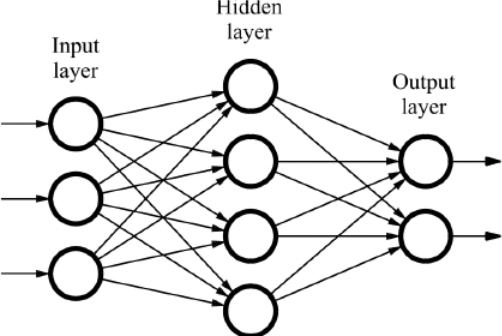
\includegraphics[width=.95\linewidth]{neural1.jpg}
    \caption{
        Neural Network
    }
    \label{fig:first-page}
\end{figure}
Machine learning has been introduced into both of the stock market and the crypto currency market to enhance investors decision making abilities, as well as help authorities to detect unsual activities on the stock market. A team made of of computer scientists and software engineering published an article in 2021 on exploring \textit{Improving stock trading decisions based on pattern recognition using machine learning technology}. They begin the pattern recognition schedule, four prominent machine learning methods and 11 different feature types are applied to all possible combinations of daily patterns, with the results being recorded in a database. To detect the prediction effect at different times of the year, several time windows ranging from one to ten days are used. An investing strategy is developed in accordance with the candlestick patterns that have been recognized and the time window that is appropriate.

Another study by Helder Sebastiao and Pedro Godinho in 2021 examined a similar topic on \textit{Forecasting and trading cypto currencies with machine learning under changing market conditions}. This study investigates the predictability of three main cryptocurrencies—bitcoin, ethereum, and litecoin—as well as the profitability of trading strategies developed using machine learning techniques. The results show that machine learning approaches are highly profitable (e.g., linear models, random forests, and support vector machines). It is possible to assess whether the models' predictions are accurate even if the market direction changes between the validation and test periods because the models are validated in a period of unprecedented turmoil and tested in a period of bear markets because the models are tested in a period of bear markets.

\textit{The anotomy of cryptocurrency Pump and Dump Scheme} by Jiahua Xu and Bejamin Livshits examines that pump-and-dump schemes have garnered the attention of both cryptocurrency observers and authorities, this article is the first to provide a full empirical examination of pump-and-dump activity in cryptocurrency markets. We present a case study of a recent pump-and-dump incident, evaluate 412 pump-and-dump actions coordinated in Telegram groups between June 17, 2018 and February 26, 2019, and identify tendencies in cryptocurrency markets related with pump-and-dump schemes. We next develop a model that forecasts the possibility of a pump occurring for all coins listed on a crypto-exchange prior to the pump. The model is highly precise and robust, and can be used to develop a simple yet highly profitable trading strategy that we demonstrate empirically can provide returns of up to 60 percent on small retail investments over a two-and-a-half month period. The study establishes a proof of concept for strategic cryptocurrency trading and gives light on the use of machine learning for criminal identification.

\section{Evaluation}

\section{Ethical Consideration}

\section{Limitations, Future Work, and Conclusion}

\section{Appendices}

\section{Conclusion}

\printbibliography 

\end{document}